We now return to the case study outlined in section \ref{sec:casestudy}. We analyze two scenarios. In figure \ref{fig:experiment}, we have 6 available mobile sensors. We compare the surveillance strategy with the situation in figure \ref{fig:3experiment} where we have only 3. Our global surveillance task is $\LTLsquare \LTLdiamond p_5$, i.e, we need to infinitely often bring the belief of the target location to 5 cells or lower. 

\begin{figure}
	\centering
\subfloat[The gridworld in \ref{fig:SGR-grid} partitioned into 6 subgames. \label{fig:experiment}]{
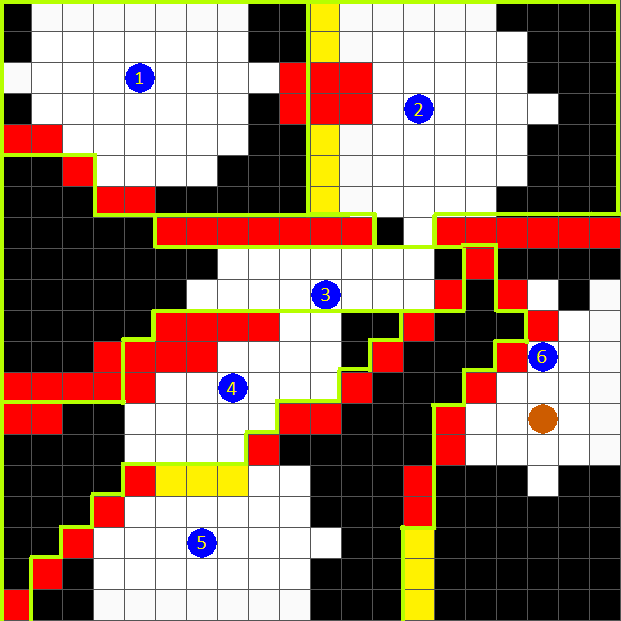
\includegraphics[scale=0.14]{figs/SGR-grid-vis-part.png}
\hspace{1.5cm}}
%\hfill
\subfloat[The gridworld in \ref{fig:SGR-grid} partitioned into 3 subgames. \label{fig:3experiment}]{
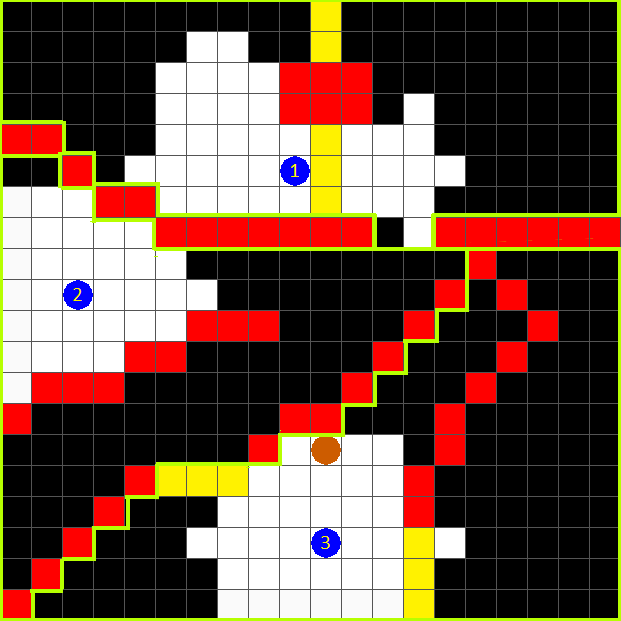
\includegraphics[scale=0.14]{figs/SGR-grid-vis-part_3.png}
\hspace{.3cm}}

\caption{We look at the case where we have 6 mobile sensors in \ref{fig:experiment} and 3 mobile sensors \ref{fig:3experiment}\label{fig:bigexp}. The mobile sensors or UAVs are blue circles and the target is represented in orange. The red cells represent impassable terrain (such as dense foliage) that cannot be seen through by the sensors. Black cells are locations not visible to any sensor.}\vspace{-0.5cm}
\end{figure} 

Solving either case centralized is not computationally feasible as the state space grows exponentially with the number of sensors. We partition the multi-agent surveillance game into subgames as shown in Figures \ref{fig:experiment} and \ref{fig:3experiment}. We then solve each game individually with local specifications $\locspec_i(\square \lozenge p_5)$

We report the synthesis times in table \ref{tab:synthtime}.

\begin{table}[h!]
	\centering
	\caption{Synthesis times for each surveillance subgame}
	\label{tab:synthtime}
	\begin{tabular}{c|l|l|l}
		\multicolumn{1}{l|}{}                                    & \textbf{Subgame} & \textbf{Number of states} & \textbf{Synthesis time (s)} \\ \hline \hline
		\multirow{7}{*}{\textbf{6 sensors}}
		& Subgame 1   & 69     & 101                          \\
	    & Subgame 2   & 74     & 206                          \\
		& Subgame 3   & 62     & 111                          \\
		& Subgame 4   & 52     & 88                          \\
		& Subgame 5   & 77     & 285                          \\
		& Subgame 6   & 66     & 64                          \\ \hline
		& \textbf{Total}   & \textbf{400}         & \textbf{855}                         \\ \hline
		\multicolumn{1}{l|}{\multirow{4}{*}{\textbf{3 sensors}}} & Subgame 1        & 142 & 473                         \\
		\multicolumn{1}{l|}{}                                    & Subgame 2        & 113 & 306                         \\
		\multicolumn{1}{l|}{}                                    & Subgame 3        & 145 & 372                         \\ \hline
		\multicolumn{1}{l|}{}                                    &  \textbf{Total} & \textbf{400}            & \textbf{1151}                        
	\end{tabular}
\end{table}

The multi-agent surveillance game in figure \ref{fig:experiment} results in more subgames compared to the game in \ref{fig:experiment}. However, each game is much smaller and strategies can be synthesized faster in each subgame. Figure \ref{fig:case1exp} shows snapshots in time of the simulation of the surveillance game in Figure \ref{fig:3experiment}. The target is being controlled by a human and the sensors in blue had local surveillance strategies synthesized. The global belief is depicted in Figure \ref{fig:case1exp} as grey cells, meaning that the combined knowledge of all the sensors has restricted the location of the target into one of the grey cells.
\begin{figure}
	\begin{minipage}{5.0cm}
		\centering
		\subfloat[$t_1$ \label{fig:case1t2}]{
			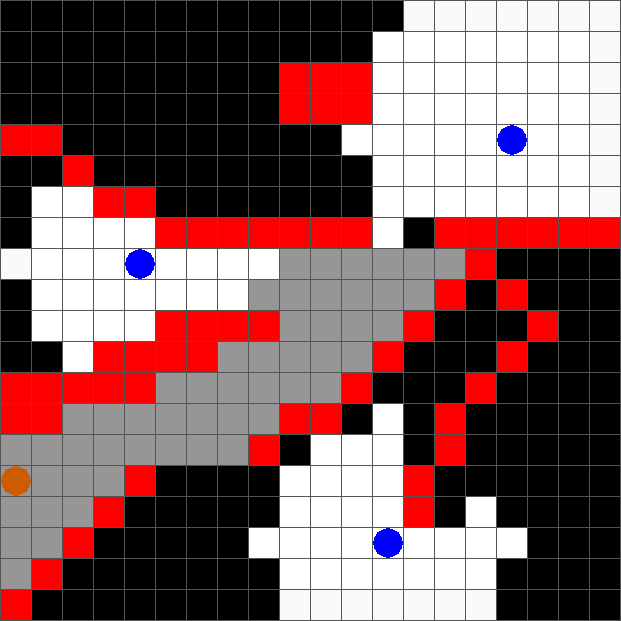
\includegraphics[scale=0.12]{figs/results_t2.png}\hspace{.5cm}
		}
		\subfloat[$t_3$ \label{fig:case1t3}]{
			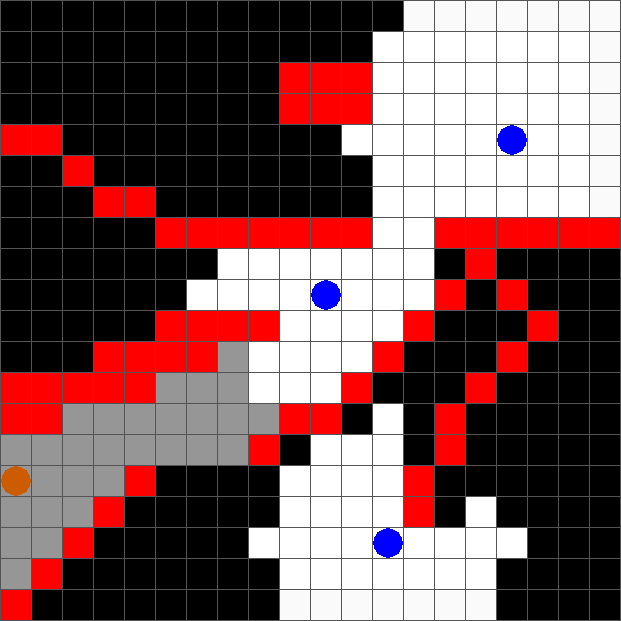
\includegraphics[scale=0.12]{figs/results_t3.png}\hspace{.5cm}
		}
		\subfloat[$t_4$ \label{fig:case1t4}]{
			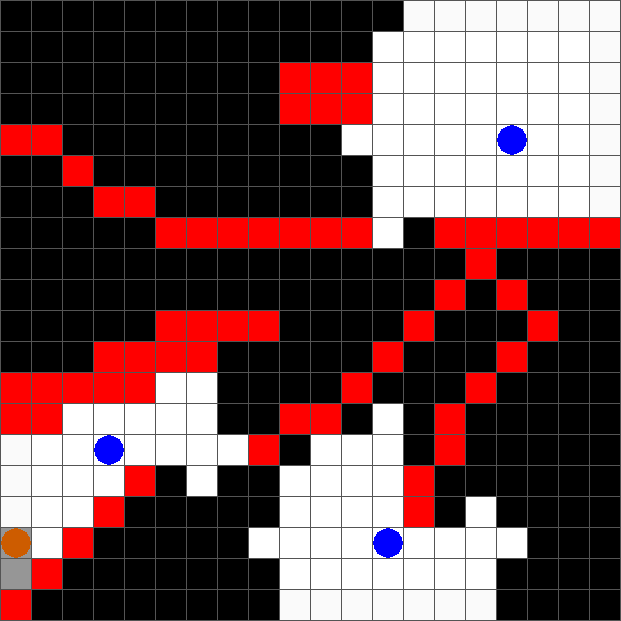
\includegraphics[scale=0.12]{figs/results_t4.png}\hspace{.5cm}
		}
	\end{minipage}
	\begin{minipage}{5.0cm}
		\centering
		\subfloat[$t_5$  \label{fig:case1t5}]{
			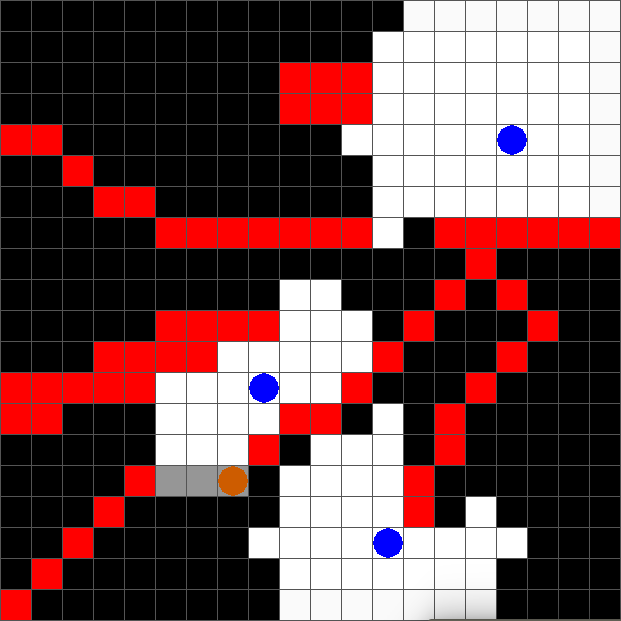
\includegraphics[scale=0.12]{figs/results_t1.png}\hspace{.5cm}
		}
		\subfloat[$t_6$ \label{fig:case1t6}]{
			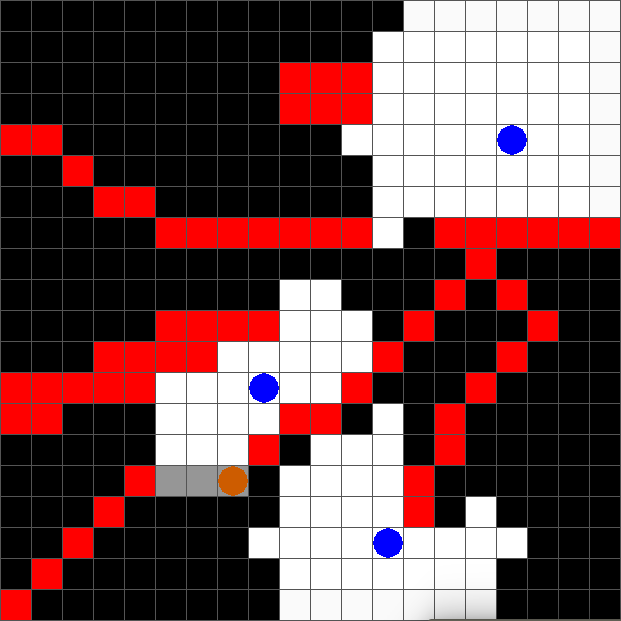
\includegraphics[scale=0.12]{figs/results_t1.png}\hspace{.5cm}
		}
		\subfloat[$t_7$ \label{fig:case1t7}]{
			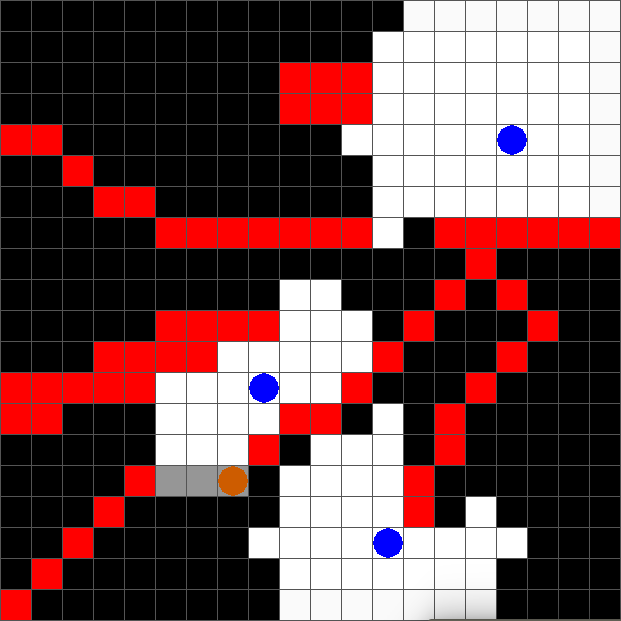
\includegraphics[scale=0.12]{figs/results_t1.png}\hspace{.5cm}
		}
		
	\end{minipage}
	
	
	\caption{Figures \ref{fig:case1t2} - \ref{fig:case1t7} are chronological snapshots at various points in time during the simulation of the surveillance game in Figure \ref{fig:3experiment}. Grey states represent the global belief of the target's location.  
	}
	\label{fig:case1exp}
	
\end{figure}

 We see that Figures \ref{fig:case1t2} - \ref{fig:case1t4}, the target is in subgame corresponding to sensor 2. Hence, only sensor two is moving and trying to lower its belief to below 5 (which it does in \ref{fig:case1t5}). In Figures \ref{fig:case1t3} - \ref{fig:case1t5}, the target moves into subgame 3 at which point sensor 3 takes over. In figure \ref{fig:case1t2}, the target is in the region of a static sensor. Hence, the global belief is restricted to the region that sensor operates. There is no communication between any of the agents - they are each only satisfying their local surveillance specification, but by our construction this guarantees that the global specification of $\square \lozenge p_5$ will be satisfied. We include a link to a video of the simulation at \url{google.com}